\documentclass{article}    % Specifies the document style.
\usepackage{color, amsmath, amsfonts, amsthm}
\usepackage{verbatim}      % For multiline comments via comment command
\usepackage{graphicx}
\renewcommand{\baselinestretch}{1}      % Spacing
\setlength{\oddsidemargin}{0in} \setlength{\evensidemargin}{0in} \setlength{\textwidth}{6.5in}
%\setlength{\topmargin}{-.2in} \setlength{\headsep}{0in} \setlength{\textheight}{9.5in}
\pagestyle{empty}
\newtheorem{proposition}{Proposition}
\newtheorem{claim}{Claim}
\newtheorem{theorem}{Theorem}
\newtheorem{definition}{Definition}
\newtheorem{lemma}{Lemma}
\newtheorem{corollary}{Corollary}
\newtheorem{example}{Example}[section]
\def\myname{(Michael) Chek Hin Choi}
\usepackage{fancyhdr}
\pagestyle{fancy}

\cfoot{}				     % no footers (in pagestyle fancy) 
\lhead{{\noindent\myname}}		     % running left heading
\rhead{{ORIE6125 Homework 1
		\quad \thepage}}%



\begin{document}           % End of preamble and beginning of text.
%\begin{center}
%\textbf{ORIE7590 Homework 1}\\[.1cm]
%\textbf{(Michael) Chek Hin Choi}
%\end{center}

\section{Floating-point arithmetics}

\begin{enumerate}
	\setcounter{enumi}{1}
	\item An example of subnormal number is $2^{-1023}$.
	
	
\end{enumerate}

\section{Cache efficiency}

\begin{enumerate}
	\item For a $12$-way associative, $6\mathrm{MiB} = 6291456$ bytes L3 cache with a 64-byte cache line, there are $6291456/64 = 98304$ cache lines, and $98304/12 = 8192$ cache blocks. Given that an int takes up $4$ bytes (in C++), each cache line can store $64/4 = 16$ integers, and each cache block has $16 \times 12 = 192$ integers. 
	
	The worst-case $npasses$ occurs when we take in each cache line, and have space in some other blocks. So the worst-case is $npasses = 16 \times 8192 n + l = 131072n + l$ where $n \in \mathbb{N}$ and $l \in \{0,1\}$.
	
	\item On my machine, it has a $16$-way associative, $8192$K bytes L3 cache with $64$-byte cache line. There are $8192 \times 2^{10}/64 = 131072$ cache lines, and $131072/16 = 8192$ cache blocks. Given that an int takes up $24$ bytes (in Python 2.7), each cache line can store $\lfloor64/24\rfloor = 2$ integers.
	
	The worst-case $npasses$ occurs when we take in each cache line, and have space in some other blocks. So the worst-case is $npasses = 2 \times 8192 n + l = 16384n + l$ where $n \in \mathbb{N}$ and $l \in \{0,1\}$.
	
	\item \text{}\\
        \begin{minipage}[t]{\linewidth}
		\centering
		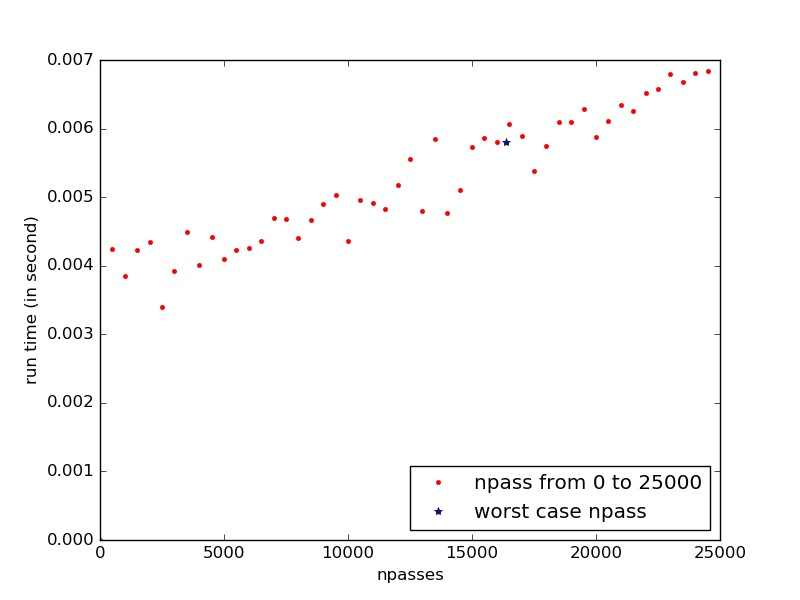
\includegraphics[width=0.5\textwidth]{cache_timing.jpg}
	\end{minipage}
	
\end{enumerate}


\end{document}

